%% generato automaticamente da tools/build_tex.py --- non modificare
\chapter{Una riga sola}
\label{cap:limit}
\quaderno{limit.dfw}{19 Dec 2009}{1}

Dicembre 2009. Il quaderno più breve della raccolta contiene una sola espressione, e non è un calcolo: è una maggiorazione. Merita un capitolo proprio perché mostra bene che cosa fossero questi file — non solo un blocco per appunti di calcolo, ma anche un posto dove fissare una disuguaglianza che era servita e che si voleva ritrovare.

\section{La disuguaglianza}
\begin{espr}{1}{User}{}
\[
\left|x\right| \leq \frac{\sqrt{2}}{2}\, \left(\frac{1}{2} + x^{2}\right)
\]
\end{espr}
A sinistra una funzione non derivabile nell'origine, a destra una parabola. La parabola sta sempre sopra e la tocca in due punti simmetrici.

\begin{figure}[htbp]
  \centering
  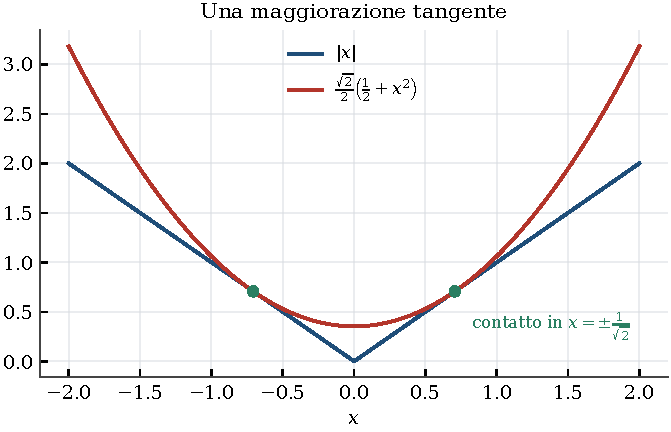
\includegraphics[width=0.86\linewidth]{../figures/limit_disug.pdf}
  \caption{La parabola $\tfrac{\sqrt2}{2}\left(\tfrac12+x^2\right)$ domina $|x|$ su tutta la retta e la tocca nei due punti $x=\pm1/\sqrt2$. La costante $\sqrt2/2$ è la più piccola per cui questo accade.}
  \label{fig:limit_disug}
\end{figure}

La disuguaglianza è vera per ogni $x$ reale e si dimostra in una riga con la media aritmetico-geometrica. Da $\left(|x|-\tfrac{1}{\sqrt2}\right)^2\geq 0$ segue $x^2+\tfrac12\geq \sqrt2\,|x|$, e moltiplicando per $\tfrac{\sqrt2}{2}$ si ottiene esattamente il secondo membro. L'uguaglianza vale nei due punti $x=\pm 1/\sqrt2$, dove la parabola è tangente alle due semirette che compongono $|x|$.

Il motivo per cui una maggiorazione di questo tipo è utile si legge nella costante: $\sqrt2/2$ è il valore più piccolo possibile. Qualunque disuguaglianza della forma $|x|\leq c\left(\tfrac12+x^2\right)$ valida su tutto $\mathbb{R}$ richiede $c\geq\sqrt2/2$, perché il rapporto $|x|/(\tfrac12+x^2)$ ha massimo $\sqrt2/2$ proprio in $x=\pm1/\sqrt2$. La costante non è scelta per comodità: è ottima.

